\documentclass[11pt, twoside, pdftex]{article}

% This include all the settings that we should use for the document
\newcommand{\PDFTitle}{Getting Started with Intel's DE-Series Boards}
\newcommand{\commonPath}{../../Common}
\newcommand{\datePublished}{Mar 2022}

\newcommand{\versnum}{21.1} %version number quartus/AMP
\newcommand{\quartusname}{Quartus\textsuperscript{\textregistered} Prime}	
\newcommand{\textBar}{For \quartusname{} \versnum{}}
\newcommand{\thisyear}{2022 } %for copyright
\newcommand{\company}{FPGAcademy.org}
\newcommand{\longteamname}{FPGAcademy.org}
\newcommand{\teamname}{FPGAcademy}
\newcommand{\website}{FPGAcademy.org}

\newcommand{\productAcronym}{AMP}
\newcommand{\productNameShort}{Monitor Program}

\newcommand{\productNameMedTM}{Monitor Program}
\newcommand{\productNameMed}{Monitor Program}

%\newcommand{\headerLogoFilePath}[1]{#1/FPGAcademy.png}



\setlength\topmargin{-0.25in}
\setlength\headheight{0in}
\setlength\headsep{0.35in}
\setlength\textheight{8.5in}
\setlength\textwidth{7in}
\setlength\oddsidemargin{-0.25in}
\setlength\evensidemargin{-0.25in}
\setlength\parindent{0.25in}
\setlength\parskip{0in} 

\pdfpagewidth 8.5in
\pdfpageheight 11in

% listings is a package that supports encapsulating source code in LaTeX conveniently

\usepackage{listings}
% add support for graphics
\usepackage{graphicx}
\usepackage[usenames, dvipsnames]{color}

\def\expandparam\lstinputlisting[#1]#2{\edef\tmp{\noexpand\lstinputlisting[#1]{#2}}\tmp}

\widowpenalty 10000
\clubpenalty 10000

%%%%%%%%%%%%%%%%%%%% Source Code Formatting %%%%%%%%%%%%%%%%%%%%
\definecolor{globalCommentColour}{rgb}{0.588,0.588,0.588}

%%%%%%%%%%%%%%%%%%%%%%%%%%%%%%%%%%%%%%%%%%%%%%%%%%%%
% Defining a NiosII ASM highlighter for lstlisting
\lstdefinelanguage[NiosII]{Assembler} {
 	morekeywords={add, addi, and, andhi, andi, beq, bge, bgeu, bgt, bgtu, ble,  bleu, blt, bltu, bne, br, break,% 
 	bret, call, callr, cmpeq, cmpeqi, cmpge, cmpgei, cmpgeu, cmpgeui, cmpgt, cmpgti, cmpgtu, cmpgtui, cmple,%
 	cmplei, cmpleu, cmpleui, cmplt, cmplti, cmpltu, cmpltui, cmpne, cmpnei, custom, div, divu, eret, flushd,%
 	flushda, flushi, flushp, initd, initda, initi, jmp, jmpi, ldb, ldbio, ldbu, ldbuio, ldh, ldhio, ldhu, ldhuio,%
 	ldw, ldwio, mov, movhi, movi, movia, movui, mul, muli, mulxss, mulxsu, mulxuu, nextpc, nop, nor, or, orhi, ori,%
 	rdctl, rdprs, ret, rol, roli, ror, sll, slli, sra, srai, srl, srli, stb, stbio, sth, sthio, stw, stwio,%
 	sub, subi, sync, trap, wrctl, wrtcl, wrprs, xor, xori, xorhi, xori},% 	
 	morekeywords=[2]{.abort, .ABORT, .align, .app-file, .ascii, .asciz, .balign, .byte, .comm, .data, .def,%
 	.desc, .dim, .double, .eject, .else, .end, .endef, .endif, .equ, .equiv, .err, .extern, .file, .fill, .float,%
 	.global, .globl, .hword, .ident, .if, .include, .int, .irp, .irpc, .lcomm, .lflags, .line, .linkonce, .ln,%
 	.list, .long, .macro, .mri, .nolist, .octa, .org, .p2align, .psize, .quad, .rept, .sbttl, .scl, .section,%
 	.set, .short, .single, .size, .sleb128, .skip, .space, .stadb, .stabn, .stabs, .string, .symver, .tag,%
 	.text, .title, .type, .val, .uleb128, .word},% 	
 	morekeywords=[3]{et, bt, gp, sp, fp, ea, sstatus, ra, pc, status, estatus, bstatus, ienable, ipending, cpuid,%
 	exception, pteaddr, tlbacc, tlbmisc, eccinj, badaddr, config, mpubase, mpuacc},% 	
 	sensitive=t,%
 	alsoletter=.,%
	morestring=[b]",%
 	morecomment=[s]{/*}{*/},%
 	morecomment=[l]\#,%
   }[keywords,comments,strings]
   
   %% NOTE: morekeywords=[2] are GNU directives.
   
   \definecolor{niosInstructionColour}{rgb}{0.000,0.608,0.000}
   \definecolor{niosDirectiveColour}{rgb}{0.000,0.000,0.902}
   \definecolor{niosSpecialRegColour}{rgb}{0.000,0.000,0.000}
   \definecolor{niosStringColour}{rgb}{0.808,0.482,0.000}
   
   %% NOTE: To make bold use: =\bfseries\color{<colour>}
   \lstdefinestyle{defaultNiosStyle} {
   language=[NiosII]{Assembler},
   stringstyle=\color{niosStringColour},
   keywordstyle=\color{niosInstructionColour},
   keywordstyle=[2]\color{niosDirectiveColour},
   keywordstyle=[3]\itshape\color{niosSpecialRegColour}
   }
%%%%%%%%%%%%%%%%%%%%%%%%%%%%%%%%%%%%%%%%%%%%%%%%%%%%

%%%%%%%%%%%%%%%%%%%%%%%%%%%%%%%%%%%%%%%%%%%%%%%%%%%%
% Defining a ArmA9 ASM highlighter for lstlisting
\lstdefinelanguage[ArmA9]{Assembler} {
 	morekeywords={ADC, ADD, ADDS, AND, ANDS, B, BAL, BEQ, BGE, BGT, BL, BLT, BIC, BKPT, BLX, BNE, BX, CDP, CLZ, CMN, CMP, EOR,%
 	EORS, LDC, LDM, LDR, LDRB, LDRBT, LDRH, LDRSB, LDRSH, LDRT, LSL, MCR, MLA, MOV, MOVW, MOVT, MRC, MRS, MSR, MUL, MVN, ORR, PLD,%
 	ROR, RSB, RSC, SBC, SMLAL, SMULL, STC, STM, STR, STRB, STRBT, STRH, STRT, SUB, SUBS, SWI, SWP, SWPB, TEQ, UMLAL,
 	PUSH, POP, MOVS, RORS, LSR},%
 	morekeywords=[2]{.abort, .ABORT, .align, .app-file, .ascii, .asciz, .balign, .byte, .comm, .data, .def,%
 	.desc, .dim, .double, .eject, .else, .end, .endef, .endif, .equ, .equiv, .err, .extern, .file, .fill, .float,%
 	.global, .globl, .hword, .ident, .if, .include, .int, .irp, .irpc, .lcomm, .lflags, .line, .linkonce, .ln,%
 	.list, .long, .macro, .mri, .nolist, .octa, .org, .p2align, .psize, .quad, .rept, .sbttl, .scl, .section,%
 	.set, .short, .single, .size, .sleb128, .skip, .space, .stadb, .stabn, .stabs, .string, .symver, .tag,%
 	.text, .title, .type, .val, .vectors, .uleb128, .word},%
 	morekeywords=[3]{SP, PC, MIDR, CTR, TCMTR, TLBTR, MPIDR, ID_PFR0, ID_PFR1, ID_DFR0, ID_MMFR0, ID_MMFR1, ID_MMFR2,%
 	ID_MMFR3, ID_ISAR0, ID_ISAR1, ID_ISAR2, ID_ISAR3, ID_ISAR4, CCSIDR, CLIDR, AIDR, CSSELR, TTBR0, TTRB1, TTBR2, DACR,%
 	DFSR, IFSR, ADFSR, AIFSR, DFAAR, IFAR, ICIALLUIS, BPIALLIS, PAR, ICIALLU, ICIMVAU, BPIALL, DCIMVAC, DCISW, V2PCWPR,%
 	DCCVAC, DCCSW, DDIMVAC, DCISW, TLBALLIS, TLBIMVAIS, TLBIASIDIS, TLBIMVAAIS, TLBIALL, TLBIMVA, TLBIASID, TLBIMVAA,%
 	PMCR, PMCNTENSET, PMCNTENCLR, PMOVSR, PMSWINC, PMSELR, PMXEVTYPER, PMXEVCNTR, PMUSERENR, PMINTENSET, PMINTENCLR,%
 	PRRR, NRRR, PLEIDR, PLEASR, PLEFSR, PLEUAR, PLEPCR, VBAR, MVBAR, ISR, FCSEIDR, CONTEXTIDR, TPIDRURW, TPIDRURO, TPIDRPRW},%
 	sensitive=f,%
 	alsoletter=.,%
	morestring=[b]",%
 	morecomment=[s]{/*}{*/},%
 	morecomment=[l]{//},%
   }[keywords,comments,strings]
   
   %% NOTE: morekeywords=[2] are GNU directives.
   
   \definecolor{armInstructionColour}{rgb}{0.000,0.608,0.000}
   \definecolor{armDirectiveColour}{rgb}{0.000,0.000,0.902}
   \definecolor{armSpecialRegColour}{rgb}{0.000,0.000,0.000}
   \definecolor{armStringColour}{rgb}{0.808,0.482,0.000}
   
   \lstdefinestyle{defaultArmStyle} {
   language=[ArmA9]{Assembler},
   stringstyle=\color{armStringColour},
   keywordstyle=\color{armInstructionColour},
   keywordstyle=[2]\color{armDirectiveColour},
   keywordstyle=[3]\itshape\color{armSpecialRegColour}
   }
%%%%%%%%%%%%%%%%%%%%%%%%%%%%%%%%%%%%%%%%%%%%%%%%%%%%

%%%%%%%%%%%%%%%%%%%%%%%%%%%%%%%%%%%%%%%%%%%%%%%%%%%%
% Defining style for the verilog.

\definecolor{verilogCommentColour}{rgb}{0.000,0.502,0.000}

\lstdefinestyle{defaultVerilogStyle} {
language={Verilog},
keywordstyle=\color{blue},
commentstyle=\color{verilogCommentColour}
}
%%%%%%%%%%%%%%%%%%%%%%%%%%%%%%%%%%%%%%%%%%%%%%%%%%%%

%%%%%%%%%%%%%%%%%%%%%%%%%%%%%%%%%%%%%%%%%%%%%%%%%%%%
% Defining style for the vhdl.
\lstdefinestyle{defaultVHDLStyle} {
language={VHDL},
keywordstyle=\color{blue},
commentstyle=\color{verilogCommentColour}
}
%%%%%%%%%%%%%%%%%%%%%%%%%%%%%%%%%%%%%%%%%%%%%%%%%%%%

%%%%%%%%%%%%%%%%%%%%%%%%%%%%%%%%%%%%%%%%%%%%%%%%%%%%
% Java
\definecolor{javaStringColour}{rgb}{0.808,0.482,0}
%%%%%%%%%%%%%%%%%%%%%%%%%%%%%%%%%%%%%%%%%%%%%%%%%%%%

%%%%%%%%%%%%%%%%%%%%%%%%%%%%%%%%%%%%%%%%%%%%%%%%%%%%
% Defining language styles
% C
\definecolor{CStringColour}{rgb}{0.808,0.482,0}
%%%%%%%%%%%%%%%%%%%%%%%%%%%%%%%%%%%%%%%%%%%%%%%%%%%%

%%%%%%%%%%%%%%%%%%%%%%%%%%%%%%%%%%%%%%%%%%%%%%%%%%%%
% Defining extended LaTeX language.
\lstdefinelanguage[LocalLaTeX]{TeX}[LaTeX]{TeX}%
 	{moretexcs={bf, it, sf, lstset},%
   	}%

\lstdefinestyle{defaultLocalLatexStyle} {
language=[LocalLatex]{TeX},
keywordstyle=\color{blue}\bfseries,
keywordstyle=[2]\color{blue},
keywordstyle=[3]\color{blue}\bfseries
}
%%%%%%%%%%%%%%%%%%%%%%%%%%%%%%%%%%%%%%%%%%%%%%%%%%%%

\lstset{
%language = C,
%language = Verilog,
%basicstyle=\color{black}\rmfamily\ttfamily,
basicstyle=\small\color{black}\ttfamily,
commentstyle=\small\color{globalCommentColour}\itshape\ttfamily,
keywordstyle=\small\color{blue}\bfseries\ttfamily,
showstringspaces=false,
frame=none, %lines % boxed listings
breaklines=true,
breakatwhitespace=true,
tabsize=4
}
%%%%%%%%%%%%%%%%%%%%%%%%%%%%%%%%%%%%%%%%%%%%%%%%%%%%%%%%%%%%%%%%


%\usepackage[centering]{geometry}.
%%%%%%%%%%%%%%%%%%%%%%%%%%%%%%%%%%%%%%%%%%%%%%%%%%%
% Document Settings
\usepackage[labelsep=period]{caption}
% we can choose a better font later
%\usepackage{palatino}
\usepackage{fourier}
%\fontencoding{T1}
% include common used symbols
\usepackage{textcomp}
% add support for graphics
\usepackage{graphicx}
\usepackage[usenames, dvipsnames]{color}
% enable to draw thick or thin table hlines
\setlength{\doublerulesep}{\arrayrulewidth}
\usepackage{longtable}
\setlongtables
%\usepackage{array}
% It may be better to use PDFLaTeX as it can generate bookmarks for the
% document

% Add some useful packages
\usepackage{ae,aecompl}
\usepackage{epsfig,float,times}

% reset the font for section
\usepackage{sectsty}
%\allsectionsfont{\fontfamily{ptm}\selectfont}
\allsectionsfont{\usefont{OT1}{phv}{bc}{n}\selectfont}

% use compact space for sections
\usepackage[compact]{titlesec}
\titlespacing{\section}{0pt}{0.2in}{*0}
\titlespacing{\subsection}{0pt}{0.1in}{*0}
\titlespacing{\subsubsection}{0pt}{0.05in}{*0}

% fancyhdr header and footer customization
\usepackage{layout}
\usepackage{fancyhdr}
\pagestyle{fancy}
\fancyhead{}
\fancyhead[R]{\textit{\tiny{\textBar}}}
\fancyfoot{}
\fancyfoot[LO,
RE]{\textrm{\href{https://www.fpgacademy.org}{\small \longteamname}} \\ {\small \datePublished }}
\fancyfoot[RO, LE]{\small \thepage}
% two-side settings
%\fancyhead{} % clear all header fields
%\fancyfoot{} % clear all footer fields
%\fancyfoot[LE,RO]{\thepage}
\renewcommand{\headrulewidth}{2pt}
\renewcommand{\headrule}{{\color{blue} \hrule width\headwidth height\headrulewidth \vskip-\headrulewidth}}
\renewcommand{\footrulewidth}{0pt}

% Format the footer on page 1
\fancypagestyle{plain}{
\fancyhead{}
\fancyfoot{}
\fancyfoot[LO,
RE]{\textrm{\href{https://www.fpgacademy.org}{\small \longteamname}} \\ {\small \datePublished }}
\fancyfoot[RO, LE]{\small \thepage}
\renewcommand{\headrulewidth}{0pt}
}
% adjust some setting to try to make the figure stay in the same page with text
% Reference: 	http://www.cs.uu.nl/~piet/floats/node1.html
%   			http://mintaka.sdsu.edu/GF/bibliog/latex/floats.html
%   General parameters, for ALL pages:
\renewcommand{\topfraction}{0.9}	% max fraction of floats at top
\renewcommand{\bottomfraction}{0.8}	% max fraction of floats at bottom
%   Parameters for TEXT pages (not float pages):
\setcounter{topnumber}{3}
\setcounter{bottomnumber}{3}
\setcounter{totalnumber}{5}     % 2 may work better
\setcounter{dbltopnumber}{2}    % for 2-column pages
\renewcommand{\dbltopfraction}{0.9}	% fit big float above 2-col. text
\renewcommand{\textfraction}{0.07}	% allow minimal text w. figs
%   Parameters for FLOAT pages (not text pages):
\renewcommand{\floatpagefraction}{0.7}	% require fuller float pages
% N.B.: floatpagefraction MUST be less than topfraction !!
\renewcommand{\dblfloatpagefraction}{0.7}	% require fuller float pages
%%%%%%%%%%%%%%%%%%%%%%%%%%%%%%%%%%%%%%%%%%%%%%%%%%%
% remember to use [htp] or [htpb] for placement
%%%%%%%%%%%%%%%%%%%%%%%%%%%%%%%%%%%%%%%%%%%%%%%%%%%

% set no indent for paragraph
\setlength{\parindent}{0em}
\addtolength{\parskip}{11pt}
\newcommand{\compact}{[topsep=0pt]}
% use this package to reduce space
\usepackage{enumitem}
\usepackage{multirow}
\usepackage{rotating}
\usepackage{pifont}
\usepackage{dingbat}
\newcommand{\itemsecond}{$\circ$}
%
%%%%%%%%%%%%%%%%%%
\date{}
\author{}
%%%%%%%%%%%%%%%%%%
\newcommand{\de}{DE-series}
\newcommand{\up}{FPGAcademy}
\newcommand{\fabric}{Avalon Switch Fabric}
\newcommand{\TODO}[1]{\textcolor{red}{\textbf{TODO}: #1}}
\def\registered{{\ooalign{\hfil\raise .00ex\hbox{\scriptsize R}\hfil\crcr\mathhexbox20D}}}

% enable url and reference(bookmarks) in pdf
\usepackage{url}
\usepackage[pdftex, colorlinks]{hyperref}
\hypersetup{%
pdftitle={\PDFTitle},
linkcolor=blue,
hyperindex=true,
pdfauthor={\longteamname},
pdfkeywords={FPGAcademy, Academic Program, Example System},
bookmarksnumbered,
bookmarksopen=false,
filecolor=blue,
pdfstartview={FitH},
urlcolor=blue,
plainpages=false,
pdfpagelabels=true,
linkbordercolor={1 1 1} %no color for link border
}%
%%%%%%%%%%%%%%%%%%%%%%%%%%%%%%%%%%%%%%%%%%%%%%%%%%%
\setlength{\fboxsep}{0.7pt}
\setlength{\fboxrule}{0.5pt}

\newcommand{\red}[1]{{\color{red}\sf{#1}}}
\newcommand{\blue}[1]{{\color{blue}\sf{#1}}}


\widowpenalty 10000

%%%%%%%%%%%%%%%%%%%%%%%%%

% Add title
\newcommand{\doctitle}{Getting Started with \newline Intel's DE-Series Boards}
\newcommand{\dochead}{Getting Started with Intel's DE-Series Boards}
% Usually no need to change these two lines

\title{\fontfamily{phv}\selectfont{\doctitle} }
\chead{ \small{\textsc{\bfseries \dochead} } }
% Customizations
%%%%%%%%%%%%%%%%%%%%%%%%%
% Allows multiple figures per page

\renewcommand\floatpagefraction{.9}
\renewcommand\topfraction{.9}
\renewcommand\bottomfraction{.9}
\renewcommand\textfraction{.1}   
\setcounter{totalnumber}{50}
\setcounter{topnumber}{50}
\setcounter{bottomnumber}{50}
\raggedbottom

%%%%%%%%%%%%%%%%%%
%%% DOCUMENT START
%\begin{document}
\begin{document}
\begin{table}
    \centering
    \begin{tabular}{p{5cm}p{4cm}}
        \hspace{-3cm}
        &
        \raisebox{1\height}{\parbox[h]{0.5\textwidth}{\Large\fontfamily{phv}\selectfont{\textsf{\doctitle}}}}
    \end{tabular}
    \label{tab:logo}
\end{table}

\colorbox[rgb]{0,0.384,0.816}{\parbox[h]{\textwidth}{\color{white}\textsf{\textit{\textBar}}}}

\thispagestyle{plain}
 
\section{Introduction}

This document introduces the Intel\textsuperscript{\textregistered} DE-series Development and Education Boards
and the supporting materials provided by Intel Corporation. 
It also explains the installation process needed to use a DE-series board
connected to a computer that has the Quartus\textsuperscript{\textregistered}  Prime CAD system 
installed on it.

Intel's DE-series Development and Education Boards have been developed to provide an
ideal vehicle for learning about digital technology in a laboratory
setting.  The DE-series boards are highly suitable for use in courses on digital logic,
computer organization, and embedded systems, as well as for design projects. 
In addition to the DE-series board and the associated software,
Intel provides supporting materials that include tutorials and laboratory exercises.
\\
\\
{\bf Contents}:
\begin{itemize}
\item Purpose of a DE-Series Board
\item Scope of a DE-Series Board and Supporting Material
\item Installation of Software and Drivers
\item Using a DE-Series Board
\end{itemize}
\clearpage
\newpage

\section{Purpose of a DE-Series Board}
University and college courses on the design of logic circuits, computer 
organization, and embedded systems usually include a laboratory component. In a modern 
curriculum, the laboratory equipment should ideally exemplify state-of-the-art technology
and design tools, but be suitable for exercises that range from the simple
tasks that illustrate basic concepts to challenging designs that
require knowledge of advanced topics. From the logistic point of view,
it is ideal if the same equipment can be used in all cases. The DE-series board
has been designed to provide the desired platform.

\section{Scope of a DE-Series Board and Supporting Material}

A DE-series board features a powerful Intel FPGA chip.
All important components on a DE-series board are connected to the pins of this chip, 
allowing the user to configure the connection between the 
various components as desired.
For simple experiments, a DE-series board includes a sufficient number of switches
(of both slide and pushbutton variety), LEDs, and 7-segment displays.
For more advanced experiments, DE-series boards include many types of peripheral devices,
such as memory chips, audio and video input/output, ethernet, USB, and so on.
For experiments that require an embedded processor, it is easy to instantiate Intel's 
Nios\textsuperscript{\textregistered}  II embedded processor, and some DE-series boards (designated as {\it SoC} boards) include
embedded processors from ARM* Ltd within the FPGA chip. 
Finally, it is possible to connect expansion boards to a DE-series board
by means of two general-purpose headers.

The main software tool needed to use the DE-series boards is the Intel Quartus Prime Lite
Edition, and the ModelSim-Intel simulator.  For processors implemented in the FPGA on a
DE-series board, software code development is facilitated by the \productNameMed{}, 
which supports both Intel's Nios II embedded processor and the ARM A9 processor in
Intel's SoC devices.  Software development is also supported 
software provided by ARM Ltd.

Traditionally, manufacturers of educational FPGA boards have provided a variety
of boards and the CAD tools needed to implement designs on these boards.
However, there has been a paucity of supporting materials that could be used
directly for teaching purposes. Intel's DE-series boards are a significant departure from
this trend. In addition to the DE-series board, Intel Corporation provides a full set
of associated exercises that can be performed in a laboratory setting for typical
courses on logic design, computer organization, and embedded systems. In effect, the 
DE-series board and the available exercises can be used as a ready-to-teach platform for such
laboratories. Of course, the DE-series board is also likely to be suitable for exercises
that have been developed for other hardware platforms and can be ported
to the DE-series platform.

\section{Installation of Software and Drivers}
The DE-series board is shipped in a package that includes all parts necessary for its
operation. The only essential parts are the power adapter and the USB cable.
There is also a protective plexiglass cover that may be used in the laboratory
environment to protect the board from accidental physical damage.

The DE-series boards require the Intel Quartus Prime CAD software. The Intel FPGA University
Program recommends installation of the version called the Quartus Prime Lite Edition. 
Install this software on the computer, and ensure that the type of Intel FPGA family 
that is used on the board is
included in the installation (the DE-series boards supported by the Quartus Prime Lite Edition
software may use the Intel Arria\textsuperscript{\textregistered} 10, Intel Max\textsuperscript{\textregistered} 10, Stratix\textsuperscript{\textregistered} IV, Stratix\textsuperscript{\textregistered} V, Cyclone\textsuperscript{\textregistered} IV, or Cyclone\textsuperscript{\textregistered} V FPGAs).
Plug in the power adapter that was included with the board. 
Use the provided USB cable to connect the connector on the DE-series board labeled
{\sf USB Blaster} to a USB port on the computer.  

Press the power button to turn on the DE-series board.
The computer will recognize the new hardware connected to its USB port, but
it will be unable to proceed if it does not have the required driver already
installed. The DE-series board is programmed by using Intel's USB-Blaster, or USB-Blaster
II, driver software.  If the driver software is not already installed, then 
follow the steps below to install the required driver.

\subsection{Installing the USB-Blaster or USB-Blaster II Driver}
\label{sec:windows_10}

The instructions below apply to computers running the Microsoft* Windows* 10 operating system. If
Microsoft Windows 7 or 8 are being used, then the equivalent (similar) steps for that system should be
followed.  

After connecting the board to the computer via USB, the window in 
Figure~\ref{fig:7} may appear to indicate that Windows does not recognize the device.  Let this window finish processing.
If a different notification appears indicating that the driver is being searched for in the 
Windows Update Web site, click the notification to open a window. Since the desired 
driver is not available on the Windows Update Web site, select the option to stop the search.

~\\
\begin{figure}[H]
	\begin{center}
		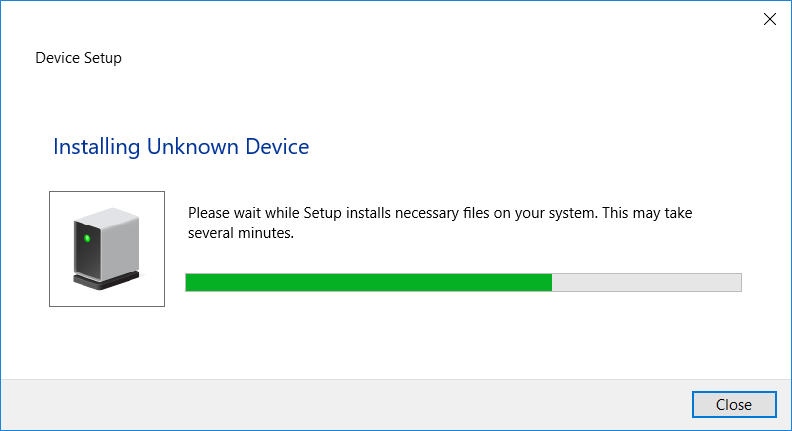
\includegraphics[scale=0.65]{figures/figure7.png}
		\caption{Notification for unsuccessful device driver installation.} 
		\label{fig:7}
	\end{center}
\end{figure}

Select {\sf Start > Control Panel > Hardware and Sound} and click {\sf Device Manager}
under {Devices and Printers} to get the window in Figure~\ref{fig:8}.  Expand the
{\sf Other devices} category and double-click the entry labeled {\sf Unknown device} to get the 
window in Figure~\ref{fig:9}. If there are multiple Unknown Devices, you may plug and unplug the DE-series board
while observing the Device Manager window to see which Unknown Device corresponds to your board. If the USB device is listed as "FT232R USB UART" rather than "Unknown Device," you may be using the wrong USB cable. Use a Type-B USB cable, which should plug in right beside the power cable, depending on the particular board.
Note that for some systems, the entry may be located at {\sf Universal Serial Bus controllers > Altera USB-Blaster}. 
Also note that if a DE-SoC board is being used, then the entry may be
labeled as {\sf USB-Blaster II} or as {\sf DE-SoC}.

\begin{figure}[H]
	\begin{center}
		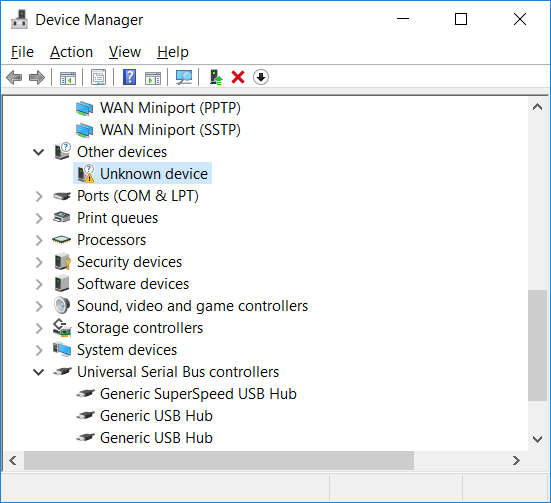
\includegraphics[scale=0.65]{figures/figure8.png}
		\caption{Click Unknown Device in the Device Manager.} 
		\label{fig:8}
	\end{center}
\end{figure}

\begin{figure}[H]
	\begin{center}
		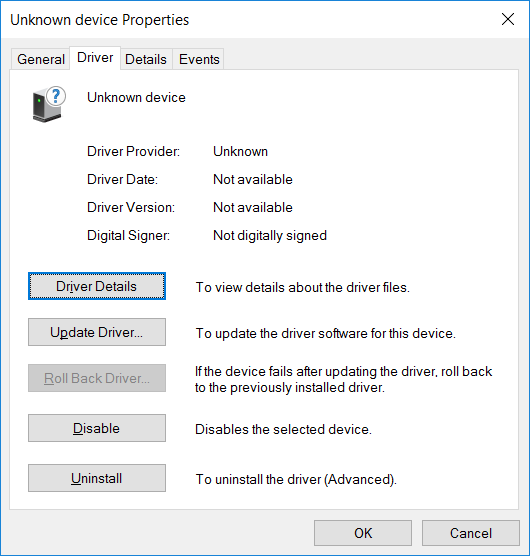
\includegraphics[scale=0.65]{figures/figure9.png}
		\caption{Click the Update Driver button.} 
		\label{fig:9}
	\end{center}
\end{figure}

In the {\sf Driver} tab select {\sf Update Driver}, which opens the window in Figure~\ref{fig:10}.
The driver is available within the Quartus Prime software.  Hence, select 
{\sf Browse my computer for driver software}.  In the window in Figure~\ref{fig:11} 
check {\sf Include subfolders} and click {\sf Browse} to get the pop-up box 
in Figure~\ref{fig:12}.

\begin{figure}[H]
	\begin{center}
		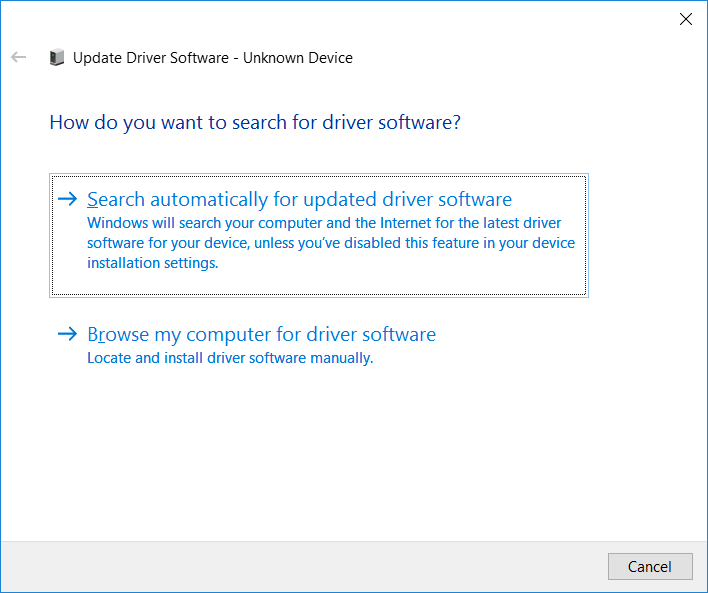
\includegraphics[scale=0.65]{figures/figure10.png}
		\caption{Browse your computer for the driver software.} 
		\label{fig:10}
	\end{center}
\end{figure}

\begin{figure}[H]
	\begin{center}
		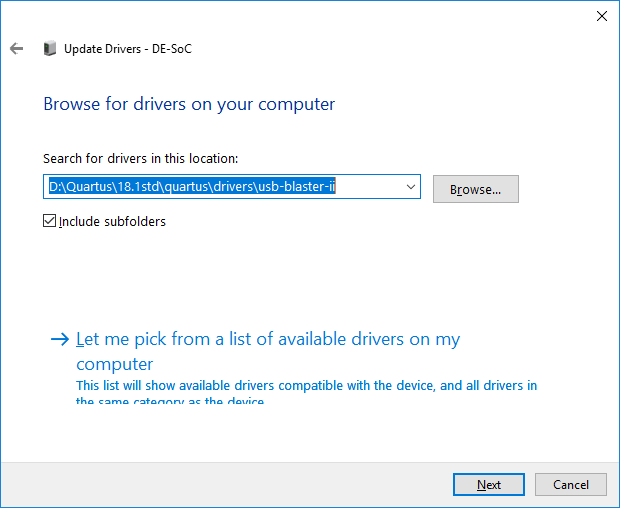
\includegraphics[scale=0.65]{figures/figure11.png}
		\caption{Specify the location of the driver.} 
		\label{fig:11}
	\end{center}
\end{figure}


Find the desired driver in your Quartus installation folder: 
{\it $\langle$QUARTUS$\_$ROOTDIR$\rangle\backslash$drivers}, where 
\linebreak
QUARTUS$\_$ROOTDIR is the Quartus Prime installation directory, such as
C:$\backslash$intelFPGA$\backslash$\versnum$\backslash$quartus.
Click {\sf OK} and then upon returning to Figure~\ref{fig:11} click {\sf Next}.

\begin{figure}[H]
	\begin{center}
		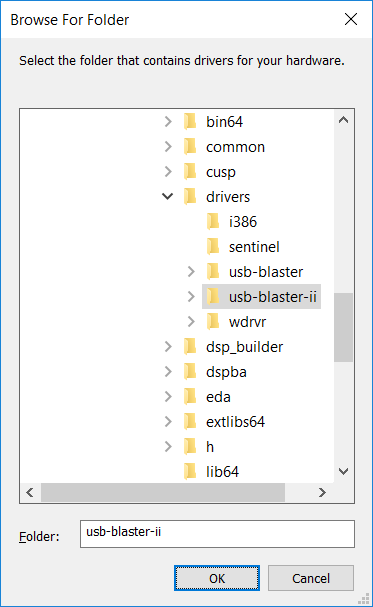
\includegraphics[scale=0.65]{figures/figure12.png}
		\caption{Browse to find the location.} 
		\label{fig:12}
	\end{center}
\end{figure}

At this point the installation will commence, but a dialog box in Figure~\ref{fig:13} may appear
indicating that Windows cannot verify the publisher of the driver software. Click {\sf Install this driver software anyway}.  The driver will now be installed as indicated in Figure~\ref{fig:14}.
Click {\sf Close} and you can start using the DE-series board.

~\\
~\\
\begin{figure}[H]
	\begin{center}
		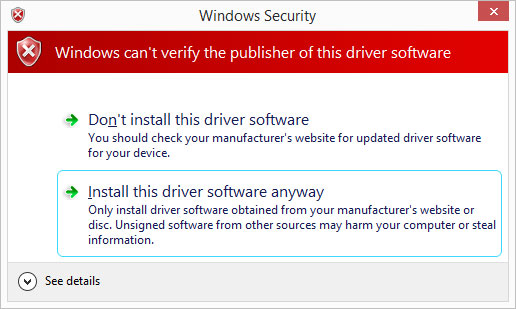
\includegraphics[scale=0.65]{figures/figure13.png}
		\caption{There is no need to verify the publisher of the driver.} 
		\label{fig:13}
	\end{center}
\end{figure}

\begin{figure}[H]
	\begin{center}
		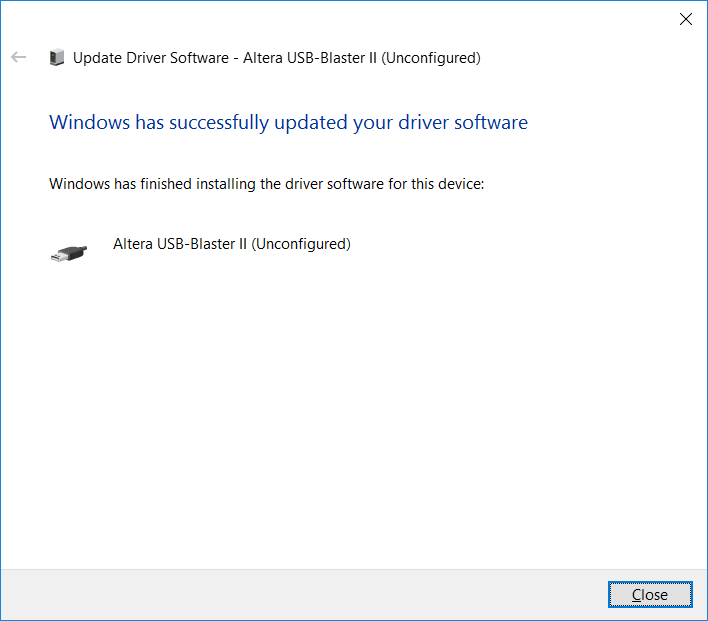
\includegraphics[scale=0.65]{figures/figure14.png}
		\caption{The driver is installed.} 
		\label{fig:14}
	\end{center}
\end{figure}

\subsection{Errors installing Driver}

You may be faced with errors causing the installation to fail, such as "Windows could not find drivers for your device" or "Windows found drivers for your device but encountered an error while trying to install them." To solve this issue, you may need to disable Device Driver Signing Enforcement. Complete the following steps to do so.

\begin{enumerate}
  \item If you computer uses BitLocker encryption, write down the recovery key (somewhere not on this computer) to use later.
  \begin{itemize}
     \item In the file explorer, right click on your hard drive.
     \item Click Manage BitLocker.
     \item Click Back up your recovery key.
     \item Click Print the recovery key, Microsoft print to PDF, then email this PDF file to another device, for instance.
   \end{itemize}
  \item Select the start menu.
  \item Open Settings.
  \item Click on Update \& Security.
  \item Click on the Restart Now button under Advanced Startup (and also remember the next few steps if you are about to restart this computer).
  \begin{figure}[H]
	\begin{center}
		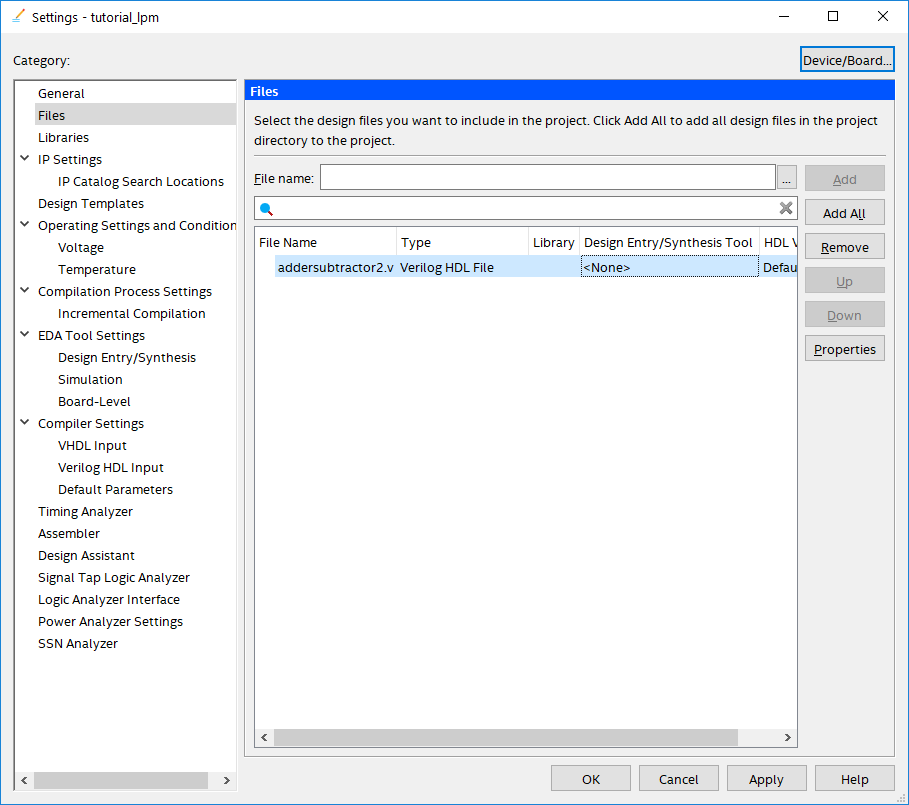
\includegraphics[scale=0.5]{figures/figure15.png}
		\caption{The settings menu before restart.}
		\label{fig:15}
	\end{center}
\end{figure}
  \item After your computer restarts, click Troubleshoot.
  \item Click Advanced options.
  \item Click Startup options.
  \item Click restart.
  \item Enter your BitLocker recovery key if/when prompted.
  \item Upon the final menu appearing, press 7 to choose Disable Driver Signing Enforcement.
\end{enumerate}

You should now be able to repeat the steps listed in section 4.1 to install the USB-Blaster or USB-Blaster II Driver with no issues.

\section{Using a DE-series Board}

A DE-series board is used in conjunction with the Quartus Prime software.
A reader who is not familiar with this software should read an introductory
tutorial. There are three versions of the tutorial:
\begin{itemize}
	\item {\it Quartus Prime Introduction Using Verilog Designs}
	\item {\it Quartus Prime Introduction Using VHDL Designs}
	\item {\it Quartus Prime Introduction Using Schematic Designs}
\end{itemize}

\noindent
Each of these tutorials cover the same aspects of the Quartus Prime software,  
differing only in the design entry method that is used.
The tutorials illustrate the entire process of implementing a design targeted
for a DE-series board.

%\newcommand{\datePublished}{Mar 2022}

\newcommand{\versnum}{21.1} %version number quartus/AMP
\newcommand{\quartusname}{Quartus\textsuperscript{\textregistered} Prime}	
\newcommand{\textBar}{For \quartusname{} \versnum{}}
\newcommand{\thisyear}{2022 } %for copyright
\newcommand{\company}{FPGAcademy.org}
\newcommand{\longteamname}{FPGAcademy.org}
\newcommand{\teamname}{FPGAcademy}
\newcommand{\website}{FPGAcademy.org}

\newcommand{\productAcronym}{AMP}
\newcommand{\productNameShort}{Monitor Program}

\newcommand{\productNameMedTM}{Monitor Program}
\newcommand{\productNameMed}{Monitor Program}

%\newcommand{\headerLogoFilePath}[1]{#1/FPGAcademy.png}



%%%%%%%%%%%%%%%%%%%%%%%%%%%%%%%%%%%%%%%%
%%% FPGAcademy Copyright Information %%%
%%%%%%%%%%%%%%%%%%%%%%%%%%%%%%%%%%%%%%%%

%Always put the copyright on a new page (clear page), with some vertical space from top
\clearpage
\vspace{1in}

\noindent

Copyright {\copyright} FPGAcademy.org. All rights reserved. FPGAcademy and the FPGAcademy logo are trademarks of  FPGAcademy.org.  This document is being provided on an ``as-is'' basis and as an accommodation and therefore all warranties, representations or guarantees of any kind (whether express, implied or statutory) including, without limitation, warranties of merchantability, non-infringement, or fitness for a particular purpose, are specifically disclaimed.

%FPGAcademy assumes no responsibility or liability arising out of the application or use of any information,  product,  or  service  described  herein  except  as  expressly  agreed  to  in  writing  by  FPGAcademy.



**Other names and brands may be claimed as the property of others.




\end{document}
